%sazeno v XeLaTeX, aby slo pismo TImes New Roman 
%nasledujici nastaveni dle BP "Sablony odbornych praci pro LaTeX"
\documentclass[12pt, twoside]{book} % vel. pisma, oboustr. tisk a typ dokumentu
\usepackage[utf8]{inputenc} % kodovani
\usepackage{cite} % citovani
\usepackage[IL2]{fontenc}
\usepackage{textgreek}
\usepackage[czech]{babel}
\usepackage{tabularx}
\usepackage[bf,sf]{titlesec}
\usepackage[top=2.5cm, bottom=2.5cm, left=3.5cm, right=2.5cm, includefoot]{geometry}
\usepackage[hidelinks]{hyperref}
\usepackage{indentfirst}
\setlength{\parindent}{10mm}
\usepackage{color}
\addto\captionsczech{
  \renewcommand{\contentsname}%
    {Contents}%
}
%%%%%%%%%%%%%%%%%%%%%%%%%%%%%%%%%%%%%%

%nasledujici baliky az po begin{document} jsou z prednastaveni sablony pro texworks
%\usepackage{geometry} % rozmery stran
%\geometry{a4paper} % or letterpaper (US) or a5paper or....
% \geometry{margin=2in} % for example, change the margins to 2 inches all round
% \geometry{landscape} % set up the page for landscape
%   read geometry.pdf for detailed page layout information
% \usepackage[parfill]{parskip} % Activate to begin paragraphs with an empty line rather than an indent
\usepackage{graphicx} % support the \includegraphics command and options
\usepackage{booktabs} % for much better looking tables
\usepackage{array} % for better arrays (eg matrices) in maths
\usepackage{paralist} % very flexible & customisable lists (eg. enumerate/itemize, etc.)
\usepackage{verbatim} % adds environment for commenting out blocks of text & for better verbatim
\usepackage{subfig} % make it possible to include more than one captioned figure/table in a single float
\usepackage{fontspec}
\usepackage[counterclockwise, figuresright]{rotating}
\usepackage{tikz}

\usepackage{floatrow}
\floatsetup[table]{capposition=top}
\floatsetup[figure]{capposition=top}

\usepackage{caption}
\captionsetup[table]{name=Table}
\captionsetup[figure]{name=Figure}

\setmainfont{Times New Roman}

%%% HEADERS & FOOTERS
\usepackage{fancyhdr} % This should be set AFTER setting up the page geometry
\pagestyle{fancy} % options: empty , plain , fancy
\renewcommand{\headrulewidth}{0pt} % customise the layout...
\lhead{}\chead{}\rhead{}
\lfoot{}\cfoot{\thepage}\rfoot{}

\addto\captionsczech{\renewcommand{\chaptername}{Chapter}}

%%% SECTION TITLE APPEARANCE
\usepackage{sectsty}
%\allsectionsfont{\sffamily\mdseries\upshape} % (See the fntguide.pdf for font help)
% (This matches ConTeXt defaults)

%%% ToC (table of contents) APPEARANCE
\usepackage[nottoc,notlof,notlot]{tocbibind} % Put the bibliography in the ToC
\usepackage[titles,subfigure]{tocloft} % Alter the style of the Table of Contents
\renewcommand{\cftsecfont}{\rmfamily\mdseries\upshape}
\renewcommand{\cftsecpagefont}{\rmfamily\mdseries\upshape} % No bold!
\renewcommand{\baselinestretch}{1.5}
%%%%%%%%%%%%%%%%%%%%%%%%%%%%%%%%%%%%%%%%%%%

\begin{document}

\begin{titlepage}   %titulni strana
\centering
\begin{center}
\textsc{ Vysoká škola ekonomická v Praze}\\[20pt]
\textbf{Národohospodářská fakulta}\\[20pt]
\textsc{Hlavní specializace: Ekonomická analýza}\\[14pt]

\begin{figure}[h]
  \centering
  
\includegraphics{obr1_nf_logo}
\end{figure}

\textsc{Are judges good at estimating the future? An application of machine learning on custody decision}\\[24pt]
\textit{diplomová práce}\\[19pt]
\vspace*{\fill}

\begin{flushleft}
\textbf{Autor: Jakub Panýr}\\[17pt] 
\textbf{Vedoucí práce:  Ing. Jan Vávra}\\[17pt]  
\textbf{Rok: 2018}\\[17pt] 
\end{flushleft}

\end{center}
\end{titlepage}

\pagestyle{empty}     %volna strana bez cislovani
\clearpage\mbox{}\clearpage


\section*{Declaration}      %prohlaseni v aj a cj
\noindent
I declare that this thesis and the work presented in it are my own and I used only sources mentioned in the References section.

\section*{Prohlášení}
\noindent 
Prohlašuji na svou čest, že jsem diplomovou práci vypracoval samostatně a s použitím 
uvedené literatury.

\vspace*{\fill}
\noindent
V Jablonci nad Nisou dne \today \hfill \dotfill

\begin{minipage}{\textwidth}
\hfill Jakub Panýr \hspace*{2.5cm}
\end{minipage} \newpage

\section*{Acknowledgment}        %podekovani v aj
\noindent I am very thankful to all people who have helped me, especially to my advisor Jan Vávra. \newpage

\section*{Assignment}           %zadani v aj
Aim of this diploma thesis is to analyze the efficiency of a pretrial custody in the Czech Republic using machine learning.\newline
Currently, there are more than 1,700 accused awaiting for trial in the Czech prisons. Taking the person into custody brings costs of imprisonment to the state and opportunity cost of social and work development to the individual. This costs should be justified by eliminating the risk of nonappearance to trial, escape or continuation in the criminal activity. Aim of this thesis is to shed light on the efficiency of the custody process represented by trade-off above and the decision making of the judges. Possible improvement of custody decision may reduce jailing rates with no change in rate of crime (or reduce crime rate with no change in jailing rate). \newline
In the theoretical part of the thesis, I will summarize the literature of judicial behavior with an accent to on custody decision. Part will conclude with a short exposition of current use of machine learning techniques in economics and their application on economics of crime. \newline
Practical part of the thesis will start by presenting summary statistics about the development and usage of the custody in the Czech Republic. Then I will closely follow the methodology used in (Kleinberg, Jon, et al. 2018), adapted to Czech context. For prediction of the custody decision and probability of re-offending or avoiding the trial, machine learning models will be formulated and selected based on predictive performance from a wide array of possible techniques. Models will be trained on micro data about custody decisions from the Czech Republic criminal system. Results from the models will be interpreted to reveal factors behind pretrial custody decision and quasi-experimental design exploiting differences between districts will be used to estimate over-usage or under-usage of custody. \newpage

\section*{Abstract}   %abstrakt v aj a nasledne v cj
\textbf{Keywords:} \newline
\textbf{JEL Classification:}


\section*{Abstrakt}
\textbf{Klíčová slova:} \newline
\textbf{JEL Klasifikace:}

\tableofcontents    %obsah
\renewcommand{\thepage}{\arabic{page}}
\renewcommand{\baselinestretch}{1.5}
\addtocontents{toc}{\protect\thispagestyle{empty}}


\chapter*{Introduction}     %uvod
\addcontentsline{toc}{chapter}{Introduction}
\pagestyle{plain}
Introduction text.


\chapter{Theoretical part}    %teoreticka cast

Zde doplnit kratounke Info o teoreticke casti, tj. co v ni bude...


\section{Literature review}     %popis literatury k tematu ekonomie zlocinu (s moznym durazem na vazbu)

Zde popis literatury (i) k tematu ekonomie zlocinu, (ii) k ML v ekonomii, (iii) k vazbe, resp. k vyuziti ML v oblasti ekonomie zlocinu (jakesi spojeni (i) a (ii))

\section{Theoretical model}    %popis literatury k tematu ML v ekonomii
 
Popis teoretickych veci (tj. napr. popis (a obrazek) rozhodovacich stromu, co je gradient boosting stromu apod.), dale vychodiska ze kterych budu vychazet (neco jako sekce III - Empirical strategy - v clanku Kleinberga). Na konec uvest teoreticky model (?).





\chapter{Practical part}        %prakticka cast

Nejprve opet na tomto miste par radku info o prakticke casti (ve stylu "nejprve prozkoumam data, pak vyhodnocuji model definovany v teor. casti, pak zkousim robustnost...").


\section{Custody in the Czech Republic}      %popisne statistiky vazby v poslednich letech s komentarem

Na toto misto doplnit popisny komentar ke grafu a tabulce; dale zdroje a zpracovani priloh a rovnez info o 
vazbe v Cr, mysleno "jak to u nas funguje" (neco se stane -> policie -> sz -> soudce -> vazba) plus odkaz na prislusne paragrafy, resp. i napriklad na vezenske rocenky ci na tu rigorozni praci. 


\begin{figure}
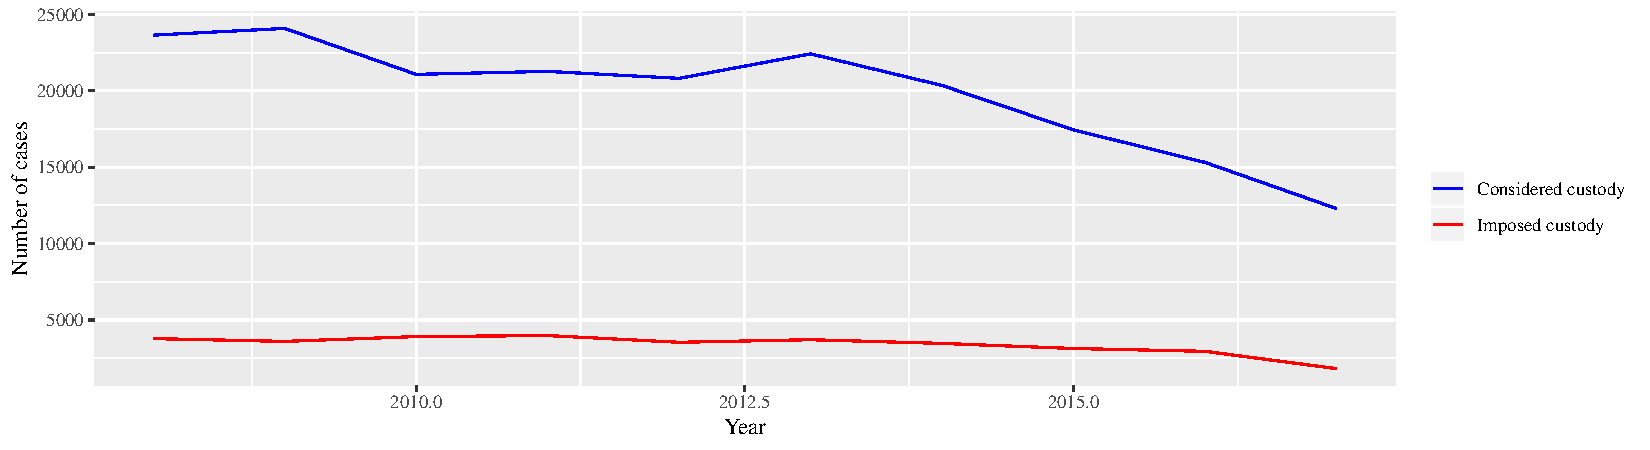
\includegraphics[width=\textwidth]{plot_21_1.pdf}
\captionof{figure}{Time evolution of number of cases handled over to a judge and of custody imposed}
Source:
\end{figure}

\newpage

\begin{sidewaystable}[H]
\centering
\begin{tabular}{rrrrrrrr}
  \hline
 Year & Possible Custody (PC) & Public Prosecution (PP) & Custody (C) & Average Length of Custody & C/PC & PC/PP \\ 
  \hline
 2008 & 23651 & 108439 & 3774 & 3.59 & 0.16 & 0.22 \\ 
   2009 & 24091 & 108599 & 3591 & 3.59 & 0.15 & 0.22 \\ 
   2010 & 21082 & 100946 & 3906 & 3.75 & 0.19 & 0.21 \\ 
   2011 & 21276 & 103624 & 3973 & 3.75 & 0.19 & 0.21 \\ 
  2012 & 20821 & 102061 & 3533 & 3.91 & 0.17 & 0.20 \\ 
   2013 & 22426 & 106507 & 3702 & 3.80 & 0.17 & 0.21 \\ 
   2014 & 20357 & 103099 & 3459 & 3.92 & 0.17 & 0.20 \\ 
   2015 & 17448 & 91357 & 3126 & 3.85 & 0.18 & 0.19 \\ 
  2016 & 15319 & 83222 & 2942 & 3.99 & 0.19 & 0.18 \\ 
   2017 & 12294 & 65184 & 1807 & 3.26 & 0.15 & 0.19 \\ 
   \hline
\end{tabular}
  \caption{Overall statistics of Custody in the Czech Republic for years 2008 to 2017 }

 \medskip
This table provides basic statistics of custody in the Czech Republic between years 2008 and 2017. Every row represents one year (captured in first column). In second column is total number of Possible Custody (PC), that is a number of cases that state prosecutor handed over to a judge, third column represents total number of cases received by Public Prosecution (PP), ratio of these two numbers (share of cases handed over from prosecutor to a judge) is then in last column. Fourth column is a total number of imposed custody for a given year, sixth column agains captures ratio, now share of custody on number of cases received by a judge. Finally in fifth column reader can find information about average length of custody in months.
\end{sidewaystable}













\section{Data}     %popisne statistiky uzitych dat s komentarem

Nejprve popis datasetu jakozto jaky je jeho zdroj atd... dale info o vycisteni a  rozdeleni na (train, test, imputation, holdout) a proc se to dela (prilozit schematicky obrazek podobny tomu v clanku Kleinberga). Dale popisne statistiky (workout setu, tj. bez holdout) s komentarem. Rovnez rozdeleni popis. stat. na ty propustene (ve smyslu vazby) a nepropustene a komentar k tomuto (zda se nejak lisi tyto dve skupiny) -  pres t-test shodnosti prumeru. Tabulka nize bude "dodelana". 


\begin{table}[ht]
\centering
\begin{tabular}{rrrr}
  \hline
 & 1 & 2 & 3 \\ 
  \hline
vazba & 0.14 & 0.00 & 1.00 \\ 
  reoff & 0.06 & 0.07 & 0.00 \\ 
  viol & 0.11 & 0.12 & 0.00 \\ 
  nonenter & 0.05 & 0.05 & 0.00 \\ 
  dmy\_vodsouz & 0.92 & 0.92 & 0.94 \\ 
  dmy\_tr\_nepo & 0.31 & 0.24 & 0.74 \\ 
  dmy\_tr\_po & 0.45 & 0.49 & 0.18 \\ 
  vek & 32.98 & 33.00 & 32.91 \\ 
  dmy\_cizinec & 0.14 & 0.14 & 0.15 \\ 
  dmy\_zena & 0.11 & 0.12 & 0.06 \\ 
  dmy\_vzd\_bez & 0.03 & 0.03 & 0.04 \\ 
  dmy\_vzd\_zakl & 0.78 & 0.78 & 0.82 \\ 
  dmy\_vzd\_str & 0.16 & 0.16 & 0.13 \\ 
  dmy\_vzd\_vys & 0.02 & 0.02 & 0.01 \\ 
  dmy\_recidivist & 0.10 & 0.09 & 0.13 \\ 
  dmy\_prv & 0.26 & 0.27 & 0.20 \\ 
  oca1 & 0.01 & 0.00 & 0.05 \\ 
  oca2 & 0.06 & 0.03 & 0.21 \\ 
  oca3 & 0.37 & 0.40 & 0.24 \\ 
  oca4 & 0.03 & 0.03 & 0.04 \\ 
  oca5 & 0.26 & 0.30 & 0.01 \\ 
  oca6 & 0.08 & 0.08 & 0.13 \\ 
  oca7 & 0.02 & 0.01 & 0.05 \\ 
  oca8 & 0.03 & 0.03 & 0.04 \\ 
  oca9 & 0.14 & 0.13 & 0.23 \\ 
  dmy\_okol\_doprava & 0.20 & 0.23 & 0.03 \\ 
  dmy\_okol\_alkohol & 0.12 & 0.13 & 0.05 \\ 
  dmy\_okol\_drugs & 0.07 & 0.05 & 0.18 \\ 
  dmy\_okol\_finance & 0.03 & 0.03 & 0.04 \\ 
  dmy\_obet\_zena & 0.10 & 0.08 & 0.24 \\ 
  dmy\_obet\_dite & 0.04 & 0.04 & 0.05 \\ 
  dmy\_obet\_muz & 0.10 & 0.09 & 0.16 \\ 
  data\_workout4 & 2013.39 & 2013.44 & 2013.05 \\ 
   \hline
\end{tabular}
\end{table}








\section{Machine learning model 1}   %model pro vyber parametru, kde y=vazba

Nejspis pres xgboost (package pro gradient boosted decision tree) a funkci important (vybere "dulezite" promenne); nasledna interpretace koeficientu u takto vybranych promennych...obecne toto zas nezabere tolik mista jako ML model2 v nasledujici subkapitole; mozno v teto sekci zkusit i treba logit a porovnat s timto ML1 modelem (viz table2 v Kleinbergovi).


\section{Machine learning model 2}     %model hodnotici, zda soudci dobre rozhoduji o vzeti do vazby

Zde tedy "hlavni" model prace, asi pres onen xgboost, kde output bude crime - porovname nejdriv predictedcrime s realnym zlocinem a zaroven i s release rate. Dale preskupim data do 4 skupin dle leniency (contracting procedure) a tim zkusim otestovat praci soudcu. Zaprve je treba test na randomprirazeni pripadu soudcum (zda treba prisnejsi nemaji jine  nez soudci benevolentni apod.), dale zda se soudci lisi v hodnoceni "unobservables", dale pak zkouset "uveznovat" dalsi lidi a porovnavat s real. soudci, zda je tam prostor pro zlepseni (shodna crime rate a vyssi release, ci shodna release a nizsi crime s uzitim algoritmu (s pomoci algoritmu) implikuje, ze tam prostor je).\newline
Pak bych, bude-li cas zkusil bych napr. test na robustnost (viz online appendix Kleinberg - jine rozdeleni datasetu, treba do roku 2015 tran a 2016+2017 test), dale test na humandatamining (to je repliakce algoritmu na holdout set (na zacatku odlozeny a netknuty)).





\chapter*{Conclusion}          %zaver
\addcontentsline{toc}{chapter}{Conclusion}

Text of a conclusion.


\bibliographystyle{unsrt}     %bibliografie s vyuzitim (v budoucnu vytvorenem) souboru "Citace"...mozna jinak, to je easy

\bibliography{Citace}



\end{document}
